\documentclass[11pt]{article}

\usepackage{amssymb,amsmath}
\usepackage{times,psfrag,epsf,epsfig,graphics,graphicx}
\usepackage{algorithm}
\usepackage{algorithmic}

\begin{document}
\date{}

\title{PHSX 343: Assignment 2}

\author{William Jardee}

\maketitle


\section*{Problem 1}

\begin{figure}[h]
    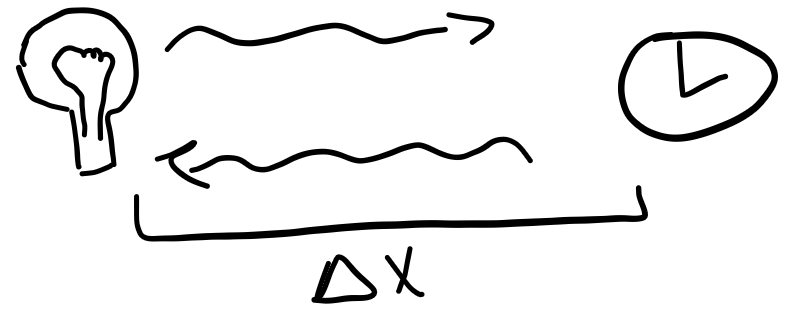
\includegraphics[width = 200 pt]{Homework2/Homework2.png}
    \label{fig:my_label}
\end{figure}
If we follow the line the light travels, we can see that it needs to take 15.0 seconds to get to my friends and another 15.0 seconds to return to me. Knowing that light travels at about $3.00x10^8 m/s$, then $\Delta x = (3.00x10^8m/s)(15.0s) = 4.50x10^8m$. The time that I see will be the time that the light reached my friend, so I will read 12:00:15. 

\section*{Problem 2}

If we state that the length of the train is L and the speed it is moving at is v; then, according to frame O, the two beams of light have to travel\\
$\Delta x_A = (\frac{1}{2}L)+V\Delta t$\\
$\Delta x_B = (\frac{1}{2}L)-V\Delta t$\\
Since the problem allows us to assume there is no time dilation, then $\Delta t$ can come from the measurement in frame O'.\\
$\frac{1}{2}L = C\Delta t \implies \Delta t = \frac{1}{2} \frac{L}{c}$\\\\
$\Delta x_A = (\frac{1}{2}L)+V\frac{1}{2} \frac{L}{c}$\\
$\Delta x_B = (\frac{1}{2}L)-V\frac{1}{2} \frac{L}{c}$\\
I we use the $\Delta t = \frac{\Delta x}{c}$ equation again, then \\
$\Delta t_A = \frac{1}{2}\frac{L}{c} + \frac{1}{2}\frac{Lv}{c^2}$\\
$\Delta t_B = \frac{1}{2}\frac{L}{c} - \frac{1}{2}\frac{Lv}{c^2}$\\
$\Delta t_A - \Delta t_B = 2(\frac{1}{2}\frac{Lv}{c^2}) = \frac{Lv}{c^2}$\\
If we then substitute in the values L=$1.00$km, v=$150.0$km/h, and c = $3.00x10^8$m/s, then $\Delta t_A - \Delta t_B = 4.64x10^{-13} s$


\section*{Problem 3}
Since we are moving perpendicularly to the separation of the two events, then any motion of the observer (or relative to the observer) is identical for the two. This meaning that the waves of the light will be compressed identically for the two events and they will stay in sync.



\end{document}
